\chapter{Introdução}

\begin{flushright}
  \textit{
    Aprender é a única coisa que a mente nunca se cansa, \\
    nunca tem medo e nunca se arrepende
  } \\
  
  \textbf{Autor desconhecido}
\end{flushright}

\section{O que é FlexBox}

O Layout do Flexbox oficialmente chamado de \textbf{Módulo de Layout de Caixa Flexível CSS} é um novo módulo de layout em CSS3 feito para melhorar os itens de alinhamento, direções e ordem no container, mesmo quando eles estão com tamanho dinâmico ou mesmo desconhecido. A principal característica do FlexBox é a capacidade de modificar a largura ou altura de seus filhos para preencher o espaço disponível da melhor maneira possível em diferentes tamanhos de tela \cite{Stojanov2015}.

Muitos designers e desenvolvedores acreditam que a disposição layout por meio do FlexBox se torna mais fácil, já que o posicionamento dos elementos é mais simples. Assim, layouts mais complexos podem ser obtidos com menos código, levando a um processo de desenvolvimento mais simples e rápido. O algoritmo de layout do Flexbox é baseado na direção, diferente do layout em bloco ou inline, que são baseados vertical e horizontalmente \cite{Stojanov2015}.

Esta nova tecnologia, hoje suportada por todos os navegadores modernos, fornece ferramentas que permitem a criação rápida de layouts complexos e flexíveis e recursos que eram difíceis com o CSS2. 

\section{Modelo do flexbox}

Antes de começarmos a descrever as propriedades do flexbox, vamos dar uma pequena introdução ao modelo do Flexbox. O layout flex é constituído pelo container pai referido como \textbf{flex container} e seus filhos imediatos, que são chamados \textbf{flex items}.

\begin{figure}[H]
  \centering
  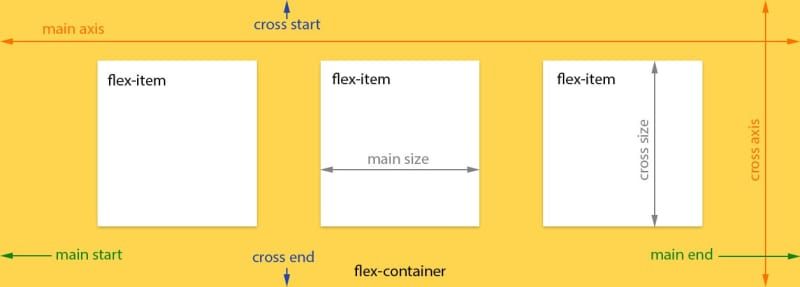
\includegraphics[scale=0.6]{imagens/CSS3-Flexbox-Model.jpg}
  \caption{Modedo do flexbox}
  \legend{Fonte: \cite{Stojanov2015}}
  \label{fig:model-flexbox}
\end{figure}

Na caixa acima, você pode ver as propriedades e a terminologia usada para descrever o conteiner Flex e seus filhos. Para mais informações sobre o seu significado, leia o modelo oficial do flexbox da W3C (https://www.w3.org/TR/css-flexbox). No próximo capítulo veremos na prática como utilizar algumas propriedade do Flexbox. 



